\section{Held-out inverse result I: emissivity-level history}\label{sec:recovery}
\subsection{Sealed design and estimator assumptions}
The first reconstruction experiment fixes $a_\star=0.5$, $i=50^\circ$, the global 224-dimensional source representation, and the registered observer schedule. The bank contains 640 histories: 256 in-class fitting-family histories, 64 in-class held-out-family histories, 256 severe off-grid fitting-family histories, and 64 mild off-grid held-out-family histories. Their records were committed before scoring. Eight paired noisy realizations accompany each history; a noiseless control is reported separately and excluded from the primary noisy endpoint. This is a finite sealed bank, not a uniform statement over every coefficient vector or every source distribution.

The primary estimators are truncated SVD (TSVD) and ridge/Tikhonov. If a whitened coefficient operator has SVD $B=U\Sigma V^T$, their spectral forms are
\begin{equation}
\widehat c_{\rm TSVD}=\sum_{s_i\geq\tau}\frac{u_i^Ty_w}{s_i}v_i,
\qquad
\widehat c_{\rm ridge}=\sum_i\frac{s_i}{s_i^2+\lambda}(u_i^Ty_w)v_i.
\label{eq:estimators}
\end{equation}
Threshold and penalty conventions belong to the individual experiment. R1 inherits its tuning from the repaired R0C validation program. HMT-2, discussed below, inherits its own stage-1 selection. Neither held-out main tunes on its test bank. These are non-Bayesian spectral estimators; their fixed source representation, known geometry, and validation-selected regularization remain substantive assumptions.

\subsection{The finite-grid field loss}
Let $D$ synthesize a reconstructed field on the source evaluation grid, and let $v_j$ be the truth evaluated on that same grid. For age $a$, normalized Gaussian weights are
\begin{equation}
\omega_{ap}=\frac{\exp[-(t_p+a)^2/(2h^2)]}
{\left(\sum_q\exp[-(t_q+a)^2/h^2]\right)^{1/2}},\qquad
W_a=\diag(\omega_{ap}),\qquad h=3M.
\label{eq:window}
\end{equation}
The registered baseline-inclusive error is
\begin{equation}
E_{jb}(a)=\frac{\norm{W_a(D\widehat c_{jb}-v_j)}_2}
{\max\{\norm{W_av_j}_2,\eta\}}.
\label{eq:r1loss}
\end{equation}
The implementation evaluates an equivalent quadratic form, detailed in Appendix~\ref{app:metrics}. It is a field loss even though the estimator and shortcut use coefficients.

The archived caller and scorer at the R1 execution commit specify $10\times12\times40=4800$ evaluation points: ten logarithmically spaced radii, twelve uniformly spaced azimuths with the repeated endpoint omitted, and forty uniformly spaced source times over \eqref{eq:referencebounds}. Spatial grid points receive equal weights in this scorer. Consequently this is a declared finite-grid scoring norm, not an independently converged approximation to a continuum physical-volume norm. It is also different from the R2 source Gram.

The floor $\eta$ is set by a fixed rule on the prior-fit split: $0.05$ times the median positive windowed truth norm, common to all test histories. Its realized numerical value was not recovered from the inspected frozen configurations, run manifest, logs, or saved summary outputs. The code path and fit-split rule are known; no replacement value is supplied here. This is a specific reproducibility limitation for the R1 normalization, not a demonstrated change in an archived endpoint or a measured assertion that the floor is harmless. Separately stored medians of absolute and normalized errors do not recover the per-evaluation denominator.

\subsection{Stable level span and negative regimes}
The primary endpoint uses \eqref{eq:stable} with $\varepsilon=0.25$, $q=0.95$, a $4M$ age grid extending to $120M$, and an $8M$ materiality floor for the paired span improvement. Uncertainty uses 10,000 paired truth-cluster bootstrap resamples, carrying all draws of a selected history together, with 95\% intervals and the frozen seed. \Cref{tab:r1} reports the archived result under that specification.

\begin{table}[htbp]
\centering\small
\caption{Stable baseline-inclusive age-local emissivity span at $\SNR=100$. Both TSVD and ridge give the stated values. The realized R1 normalization-floor scalar is not located in the inspected records; these are retained archived endpoints, not a new exact reproduction.}
\label{tab:r1}
\begin{tabular}{l r r r r}
\toprule
Regime&Histories&Direct ($M$)&Labelled ($M$)&Difference ($M$)\\
\midrule
In-class, fitting families&256&48&80&32\\
In-class, held-out family&64&48&80&32\\
Mild off-grid, held-out family&64&48&80&32\\
Severe off-grid, fitting families&256&0&0&0\\
\bottomrule
\end{tabular}
\end{table}

The positive span gain is four times the declared materiality floor. It occurs in the two in-class regimes and the mild-mismatch diagnostic. Severe mismatch remains negative. The bank size of 640 must not be described as 640 uniformly successful histories, nor may a fitting-family breakdown replace the regime table.

The endpoint is strongly level dominated. The recorded level fraction is approximately $0.9838$ under the experiment's level/structure decomposition. At the reference SNR, the archived all-age level errors are $0.266$ direct and $0.028$ labelled; the all-age structure errors are $0.927$ and $0.466$. In the old band the corresponding level errors are $0.653$ and $0.217$, whereas structure errors remain $1.169$ and $1.141$. These diagnostics show why improved baseline-inclusive level history cannot be relabelled old-morphology recovery.

The structure-only stable span is zero for both physical arms at $\SNR=100$. In the reported high-SNR study it first becomes nonzero at $\SNR=30000$, with $40M$ direct and $76M$ labelled. This onset is not lowered by adding the orders. A separate localized-source validation at $\SNR=1000$ meets an aggregate structural-materiality criterion while retaining zero stable-span gain; it is not the same endpoint or a sealed main replacing the $30000$ result. No observational exposure-time forecast is inferred from these operator-normalized SNR values.

Posterior-calibration criteria failed in the R1 probabilistic estimator branch, so calibrated posterior uncertainty is not claimed. This withdrawal is distinct from the use of TSVD and ridge as point estimators and from the bootstrap uncertainty on an empirical performance statistic.

\section{Held-out inverse result II: resolution-aware morphology}\label{sec:morphology}
\subsection{Specify the historical object before scoring it}
A pixelwise error can ask for details that neither the source representation nor the evaluation grid resolves. The morphology program therefore specifies the source object before comparing observation arms. A source-only audit over 169 sources and three refinement grids distinguished resolved pairs, stable blends, and topology-ambiguous states. In that audit, projection into the original contrast representation merged 29.9\% of stably multi-resolved pairs; radial enrichment reduced the rate to 13.6\%. These are representation diagnostics, not reconstructions from light.

Every truth--age state is assigned one of five reconciled labels: single resolved, multiple resolved, blended, dead, or ambiguous. The label selects a loss appropriate to the resolved object. Resolved states use unbalanced feature-set assignment so that missing or invented features incur an error. Blended and ambiguous states use centroid, size, azimuthal-mode, and contrast descriptors. Dead states use amplitude. Every state contributes to the primary endpoint; a difficult state is not dropped to improve the result. The explicit branch formulas are summarized in Appendix~\ref{app:morphloss}.

Two targets are kept separate. The \emph{class-conditional} target is the best in-class source object and isolates estimation error from representation mismatch. The \emph{analytic-source} target includes both mismatch and inversion error. The latter is called \texttt{PHYSICAL\_END\_TO\_END} in the archive; here it means fidelity to an analytic source within the simulation, not an instrumental or continuous-quadrature validation.

\subsection{Sealed main and paired aggregation}
The sealed main uses the same reconstruction geometry, 60 histories from six families, four paired noise draws per history, and the primary nominal 896-dimensional radial-enriched class with 768 active contrast coefficients. This reduced scope was fixed before the new bank was generated; it is not the earlier 96-history/eight-draw authorization. The contemporaneous record supplies no reason for the reduction, so no retrospective resource explanation is asserted. Its principal statistical consequence is limited family-level precision.

For a fixed class, estimator, target, and SNR, write $e_{jbak}$ for the state-dependent error at age $k$, draw $b$, arm $a$, and history $j$. The caller aggregates as
\begin{equation}
\bar e_{ja}=\frac{1}{N_b}\sum_b\left(\frac{1}{N_a}\sum_k e_{jbak}\right),\qquad
r_j^{(a)}=\frac{\bar e_{j,\rm direct}-\bar e_{ja}}
{\max\{\abs{\bar e_{j,\rm direct}},10^{-300}\}},\qquad
\widehat R_a=\med_j r_j^{(a)}.
\label{eq:hmtestimand}
\end{equation}
Histories are paired by their fixed identifiers. The primary statistic is the median of history-level relative reductions \emph{after} within-history averaging, not the relative reduction of two population means or the median of individual state ratios. The history is the independent bootstrap unit. The median's 95\% percentile interval uses 10,000 resamples at the recorded helper seed 20260954. A separately computed family-balanced mean is not substituted for the primary estimand.

Materiality was fixed at a median reduction of at least $0.10$ and a lower 95\% bootstrap endpoint of at least $0.05$. The reported main pairing contains 60 histories. The recorded paired-score filter and population are retained; this revision does not independently re-score or certify the absence of missing pairs.

\begin{table}[htbp]
\centering\small
\caption{Primary HMT-2 median paired morphology-error reductions at $\SNR=100$. The lower endpoint is from the registered 95\% history-bootstrap interval. The analytic-source target combines representation and inversion error within the simulation; it is not physical acquisition validation.}
\label{tab:hmt2}
\begin{tabular}{l l r r}
\toprule
Target&Estimator&Median reduction&95\% lower endpoint\\
\midrule
Analytic source&TSVD&0.133&0.101\\
Analytic source&Ridge&0.164&0.116\\
Class conditional&TSVD&0.160&0.092\\
Class conditional&Ridge&0.158&0.114\\
\bottomrule
\end{tabular}
\end{table}

All four primary entries in \cref{tab:hmt2} satisfy both floors. The non-dead analytic-source companions remain material, with median reductions $0.142$ for TSVD and $0.158$ for ridge. The all-order total-flux readout does not reproduce the material gain. The index-sum compression reaches at most $0.015$ with a negative lower bound. The latter is a result about that constructed compression only: no conclusion about a physically unresolved spatial image follows from it.

\begin{figure}[htbp]
\centering
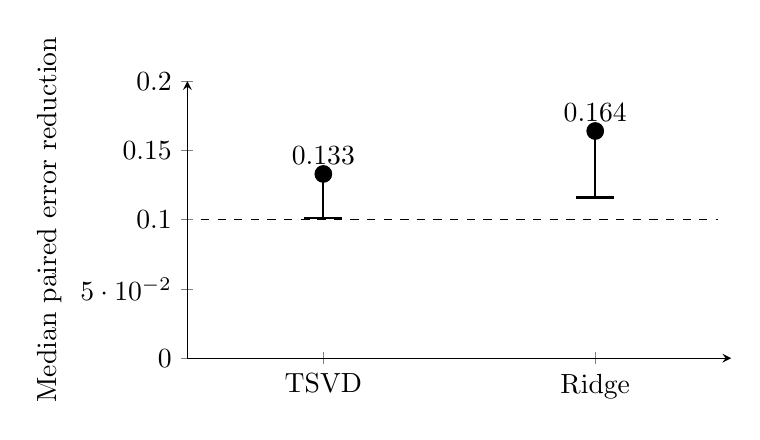
\begin{tikzpicture}
\begin{axis}[width=0.70\linewidth,height=5.1cm,xmin=0.5,xmax=2.5,ymin=0,ymax=0.2,
xtick={1,2},xticklabels={TSVD,Ridge},ylabel={Median paired error reduction},
axis lines=left,ytick={0,0.05,0.10,0.15,0.20},clip=false]
\addplot[black,dashed,domain=0.55:2.45]{0.10};
\addplot[only marks,mark=*,mark size=3pt,black] coordinates {(1,0.133)(2,0.164)};
\addplot[black,thick] coordinates {(1,0.101)(1,0.133)};
\addplot[black,thick] coordinates {(2,0.116)(2,0.164)};
\addplot[black,thick] coordinates {(0.93,0.101)(1.07,0.101)};
\addplot[black,thick] coordinates {(1.93,0.116)(2.07,0.116)};
\node[anchor=south] at (axis cs:1,0.133){0.133};
\node[anchor=south] at (axis cs:2,0.164){0.164};
\end{axis}
\end{tikzpicture}
\caption{Analytic-source morphology endpoint. Markers show median history-level paired reductions; stems terminate at the reported lower 95\% endpoints, not full two-sided error bars. The dashed line is the $0.10$ point-estimate materiality floor; both lower endpoints also exceed the separate $0.05$ requirement. These two estimators use the same paired history bank and are not independent experiments.}
\label{fig:morphology}
\end{figure}

\subsection{Four qualifications and a separate class comparison}
\paragraph{Family heterogeneity.}
Five of twelve family--estimator cells are material on the analytic-source target and four of twelve on both targets. The largest reported effects occur for flare birth--motion--decay and the structural-mode family. The simplest circular-hotspot family is negative under both estimators, with median reductions $-0.022$ for ridge and $-0.051$ for TSVD. Ten histories per family yield wide intervals. The aggregate is a result over a heterogeneous bank, not a uniform source-family law.

\paragraph{Multi-feature recovery.}
No stable multi-resolved family--estimator cell reaches materiality. The reported unbalanced assignment costs are approximately $1.21$--$1.30$, with a cost of one corresponding to a whole unmatched feature under that diagnostic. Improving an aggregate state score is therefore not reliable recovery of a resolved pair of historical tracks.

\paragraph{Stable morphology interval.}
For every arm, estimator, class, and tested SNR in this program, the stable morphology interval at $(\varepsilon,q)=(0.25,0.95)$ is zero. At reference SNR, mean within-tolerance reach is slightly lower for the labelled arm than the direct arm ($3.06M$ versus $3.32M$); the ordering reverses at tenfold SNR ($3.45M$ versus $2.92M$). Neither yields a nonzero 95\%-reliable contiguous morphology interval. Mean improvement and a reliable movie segment remain different outcomes.

\paragraph{Baseline saturation.}
Approximately 55--57\% of direct-image states are at the morphology metric ceiling. The labelled arm reduces catastrophic failures, while its absolute all-state error remains about $0.60$--$0.65$ on a scale capped at one. The improvement is meaningful relative to that baseline but is not generally accurate source recovery.

Class dependence is a separate comparison, not family heterogeneity. In the smaller nominal 448-dimensional contrast class, the analytic-source TSVD gain is $0.061$ with lower endpoint $0.033$, below the materiality requirements. The richer-class result is therefore conditional on the declared source resolution. None of these estimator outcomes is a reconstruction of the two nuisance-adjusted R2 modes: the targets, norms, and nuisance/background treatments are different experiments.
\FloatBarrier
